\documentclass[12pt]{article}
\usepackage{lingmacros}
\usepackage{tree-dvips}
\usepackage{datetime}
\usepackage{color}
\usepackage{graphicx}
\graphicspath{ {images/} }
\title{Master thesis proposal}
\author{Ion Madrazo Azpiazu}
\date{\today}
\begin{document}


\maketitle
\section{Introduction}
\begin{itemize}
\item \textbf{Context} What is a readability score?
\item \textbf{Audience} Searching books at suitable comprehension levels for children or for language learners. Teachers would be the main stakeholders here, since they would get the most benefit of a tool that would help them obtaining new materials and for curriculum design. Automatic text simplification, for summary generation, for people with reading difficulties. Literacy assessment. Political or medical document complexity assessment. 
\item \textbf{What is the problem?} 
\begin{itemize}
\item Historically used metrics are not precise enough. They base they work on very simple or shallow features, such as word length or sentence length.
\item Tools developed for readability prediction are usually monolingual. They tend to be monolingual because the tools and datasets used are so too.
\end{itemize}  
\item \textbf{What do we propose?} An exploration of new features that fit most of the languages and that fit specific languages. A multilingual tool that is able to detect the input language on the fly and use the best set of features for that specific language for prediction. {\color{red}Why isn't monolingual enough?}

\item \textbf{In doing so we will contribute to}
\begin{itemize}
\item \textbf{An application} that will help people with different profiles in selecting texts and books in different languages.
\item \textbf{An analysis} of current tools and methods developed.
\item \textbf{Several datasets}, that will be created as a byproduct of the development and the testing of the applications. 
\end{itemize}

\item \textbf{Case study} Even if the application will be able to work in many more languages, for practical purposes, the application will be tested in three different languages. English, for state of the art comparison purposes and as reference of germanic languages. Spanish, as a reference for latin languages, and Basque as an example of a non-indoeuropean language.

\end{itemize}

\section{Thesis statement}
\begin{itemize}
\item Develop a survey of currently used readability tools and methods
\item Develop a multilingual readability predictor taking advantage of machine learning techniques and features extracted using natural language processing techniques.
\end{itemize}

\section{Related work}
\subsection{Historical readability measures}
Description of basic readability scores. When and where were they used? Fleisch etc...
\subsection{General State of the art}

\subsection{State of the art for English}
\subsection{State of the art for Spanish}
\subsection{State of the art for Basque}

\subsection{State of the art for multilingual predictors}

\section{Methodology}
The proposed method relies in two different areas of data science, Natural language processing and machine learning. Advantage of one or both areas is taken in each of the steps that conform the pipeline of the algorithm explained below.
\subsection{Pipeline description}
The pipeline of the algorithm if composed by the following steps: Texts processing, feature extraction, feature processing and prediction. A visual description of the general pipeline of the system can be seen on figure \ref{fig:pipeline}.  A more in-depth explanation of each step can be seen in the following sections.

\begin{figure}[h]
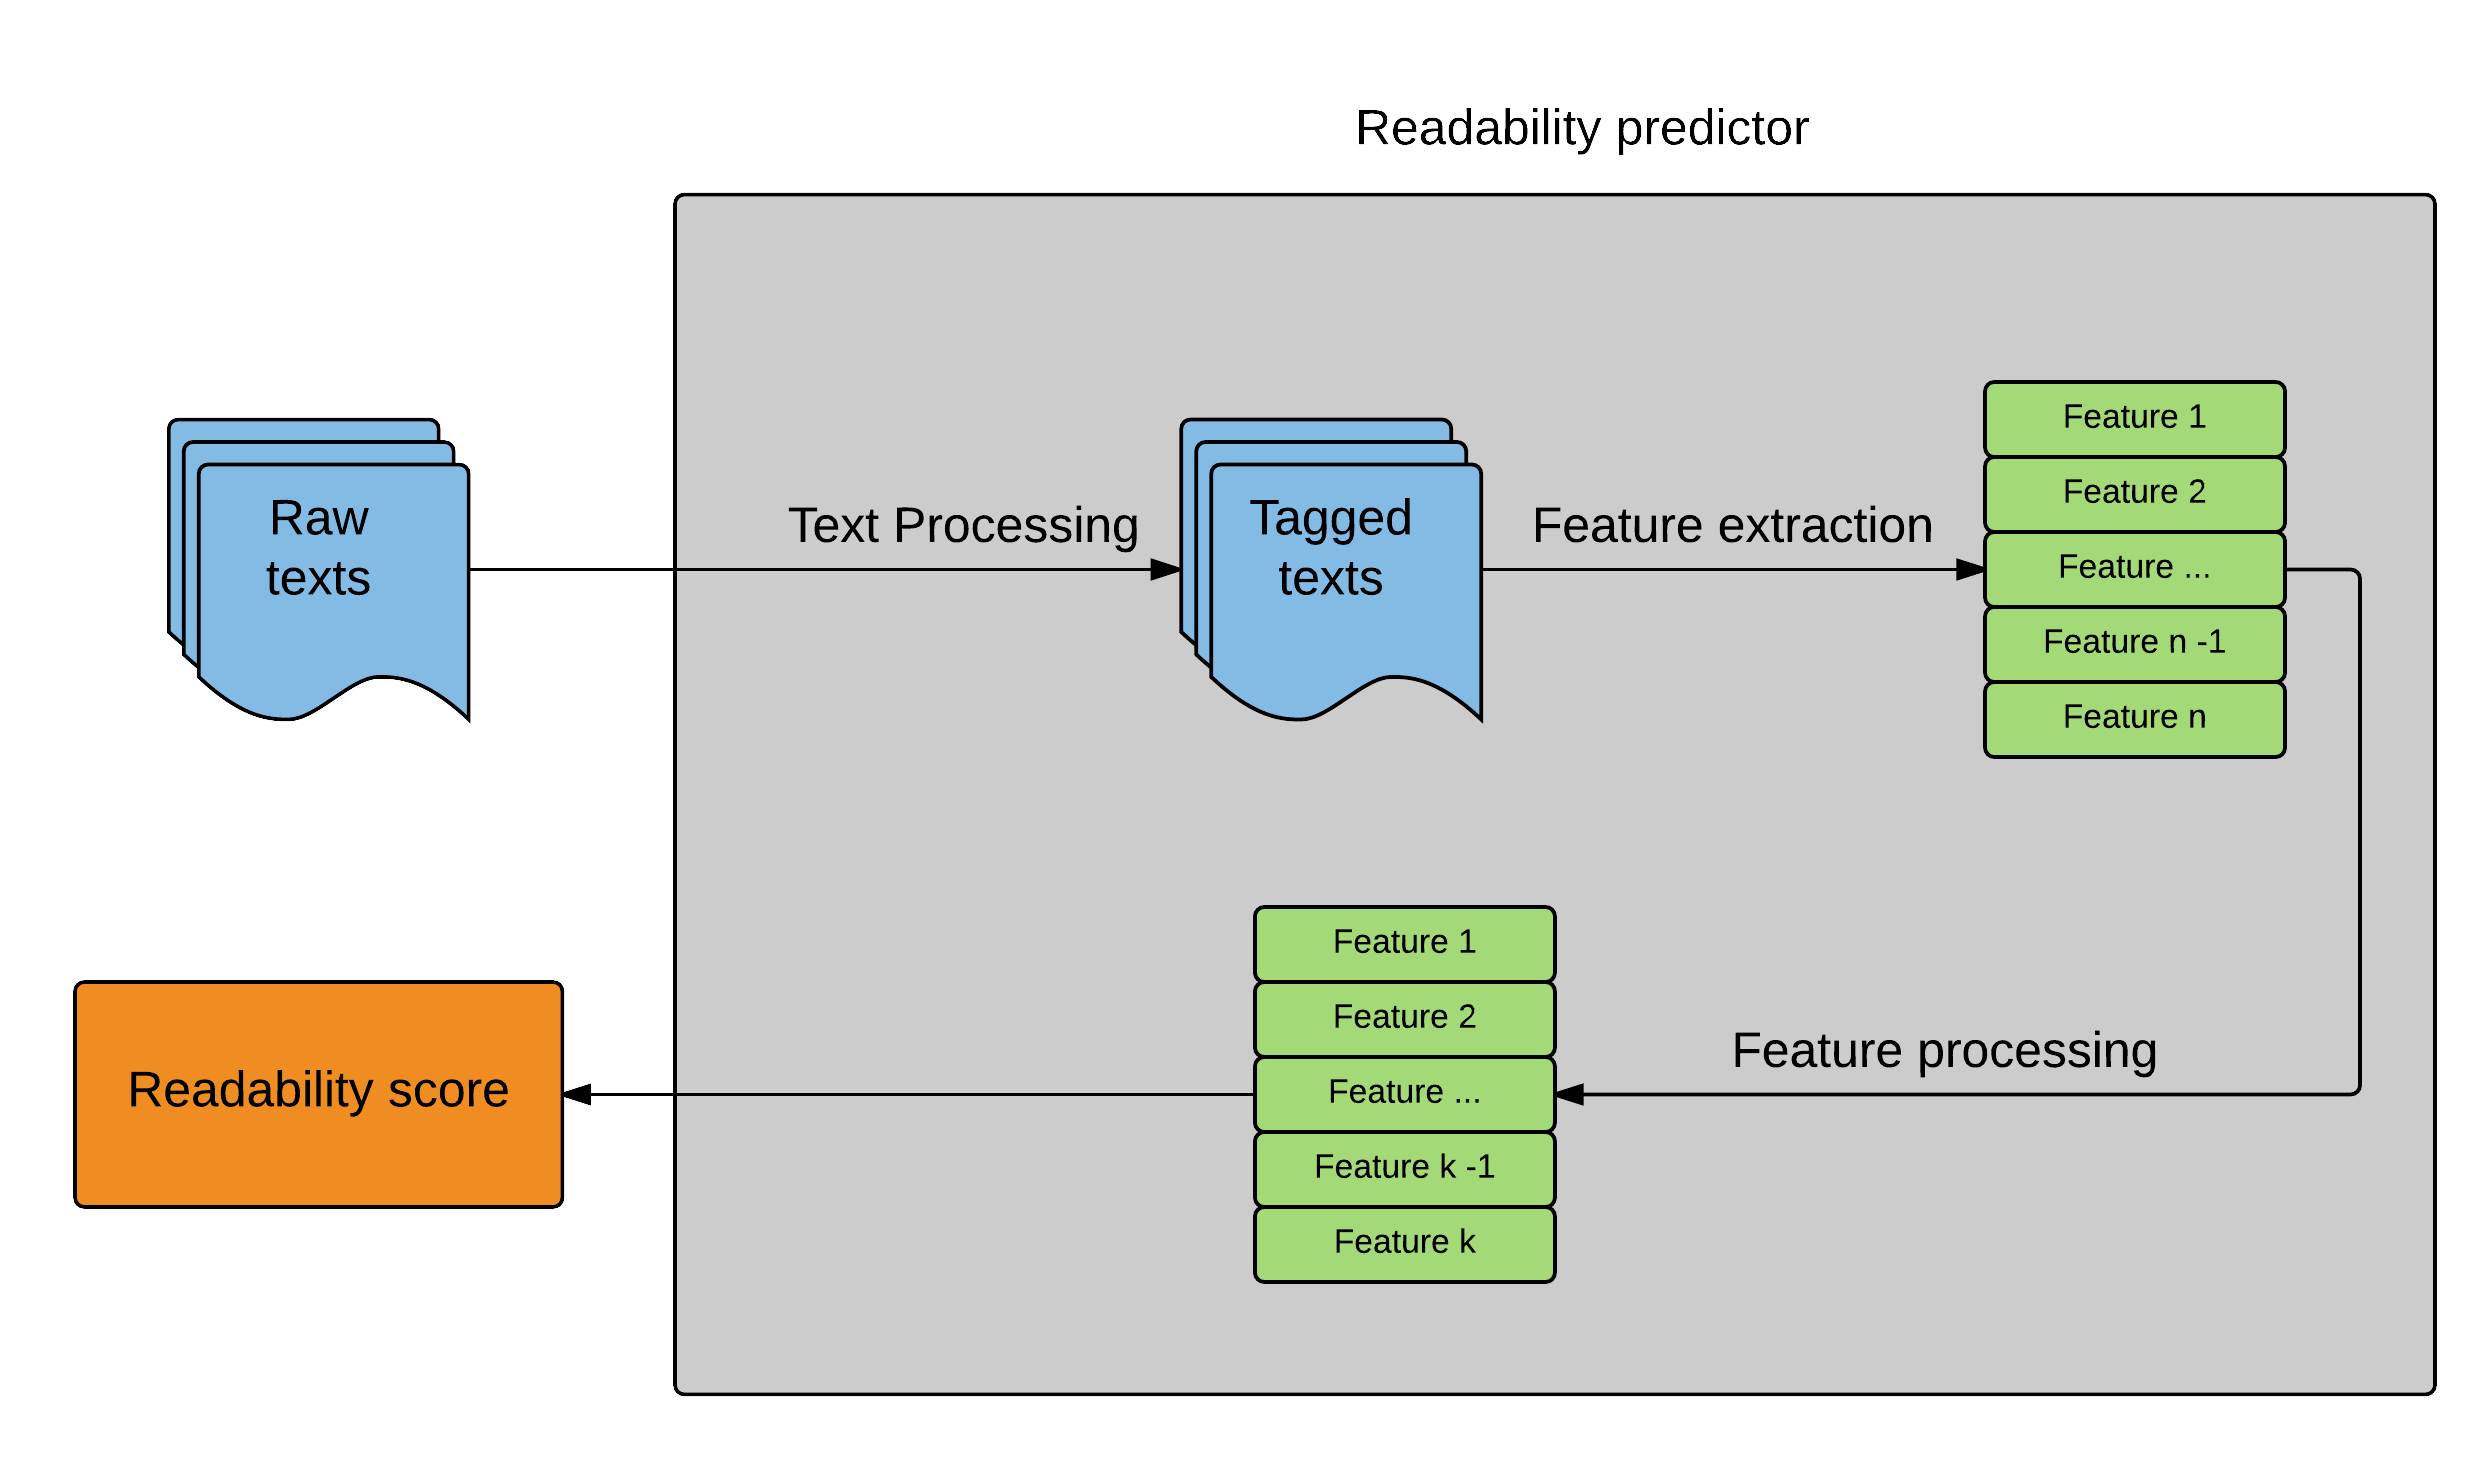
\includegraphics[width=\textwidth]{pipeline}
\caption{General pipeline}
\label{fig:pipeline}
\end{figure}

\subsection{Text processing}

The text processing step is the step where the raw text is given structure and, therefore, value. This structure and information will later be used for extraction features that will help the system predict a readability score.\\

The tool that has been chosen for natural language processing is Freeling NLP\cite{freelingNLP}. Freeling is an open source Natural language processing library that supports 11 different languages. The tool solves common NLP tasks, such as, Tokenization, sentence detection, Part of speech tagging or dependency parsing. Each of this processes will be helpful for building certain features later. A description of each module and a reasoning about why it is used is detailed next.\\

The \textbf{tokenization} module is the base module for any NLP processing...

The \textbf{Part of speech} module determines the function each token has in the sentence...

Which tool are we going to use? Why Freeling? Description of Freeling NLPTools, which modules are we using. Description of each module with a general description and examples. Generate hypotheses of why this module should add valuable information to the text.

\subsection{Feature extraction}
Description of all the features used. Why should this feature be valuable, give hypotheses and intuition behind the use of each feature. Give examples when needed.

\subsection{Feature processing and selection}
Describe algorithms used for feature processing and selection, why should they help get better results?

\subsection{Learning and prediction}
Describe algorithms for learning and prediction. Pros an cons of each algorithm, why should this algorithm adapt better to our problem?

\section{Evaluation}

\subsection{Datasets}
Information about how we get and extract the datasets.
\subsubsection{English}
\begin{itemize}
\item Lexile
\item List all for proposal...
\end{itemize}
\subsubsection{Spanish}
\begin{itemize}
\item Lexile
\item List all for proposal...
\end{itemize}
\subsubsection{Basque}
\begin{itemize}
\item Ikasbil
\end{itemize}

\subsection{Metrics}

\begin{itemize}
\item Error rate, accuracy
\item Adjacent accuracy, double adjacent accuracy...
\item Average error distance
\end{itemize}

\subsection{Tests}

\begin{itemize}

\item Which features add the most value? Correlation, information gain etc.

\item Do features correlate similarly with the readability score for each language?

\item Feature preprocessing, does it help?
	\begin{itemize}
	\item Discretization
	\item Feature subset selection techniques
	\end{itemize}
	
\item Comparison of learning models, which learning model fits best the problem?
	\begin{itemize}
	\item KNN
	\item Bayesian models
	\item SVM
	\item Neural network
	\item Regression (Adding a sense of order in class values)
	\item Ordinal classification (Adding a \textbf{stronger} sense of order in class values)
	\end{itemize}

\item \textbf{Comparison} of the system vs \textbf{baselines} such as fleish for each language individually.

\item Comparison \textbf{vs state of the art} systems for each language.

\item Multi vs monolingual
\item If we take a bilingual corpus, does the system predict same values? And if we take a text and translate it to another language? Does the readability values mantain using an automatic translator?
\end{itemize}

\end{document}